%
% hermite.tex
%
% (c) 2020 Prof Dr Andreas Müller, Hochschule Rapperswil
%
\section{Hermite-Interpolation
\label{buch:section:hermite}}
\rhead{Hermite-Interpolation}
Das Lagrange-Interpolationspolynom nimmt zwar in umittelbarer Nähe der 
Stützstellen zuverlässig Funktsionswerte nahe den gegeben Werten an,
doch insbesondere gegen den Rand des Intervals können die oft beobachteten
Oszillationen eine schlechte Approximation bewirken.
Im Gegensatz zur Taylorreihe, deren Ableitung mindestens in der Nähe des
Entwicklungspunktes auch mit der Ableitung der zu approximierenden
Funktion übereinstimmt, gibt es für das Interpolationspolynom keine
solche Garantie.
Beide Schwierigkeiten könnten gemildert werden, indem gefordert wird,
dass das Polynom nicht nur die gleichen Funktionswerte, sondern auch
die gleichen Ableitungen bis zu einer bestimmten Ordnung haben soll.
Dies ist die Idee der {\em Hermite-Interpolation},
\index{Hermite-Interpolation}%
die in diesem Abschnitt vorgestellt werden soll.

%
% Aufgabenstellung
%
\subsection{Aufgabenstellung
\label{b8ch:subsection:hermite:aufgabe}}
Das Hermite-Interpolationspolynom löst die folgende Approximationsaufgabe.

\begin{aufgabe}[Hermite-Interpolationspolynom]
Gegeben Stützstellen
\[
a=x_0<x_1<x_2<\dots < x_{n-1}<x_n=b
\]
und Funktionswerte $f_i$, $0\le i\le n$, und Werte
$s_i^{(k)}$ der $k$-ten Ableitungen bis zur $m$-ten Ordnung, $1\le k\le m$,
finde ein Polynom $h$, mit
\begin{equation}
h(x_i) = f_i,\quad h^{(k)}(x_i)=s_i^{(k)},\quad 0\le i \le n, 1\le k\le m.
\label{buch:equation:hermitebedingungen}
\end{equation}
\end{aufgabe}
Die Aufgabenstellung formuliert $N=(n+1)(k+1)$ Bedingungen für das Polynom $h$,
es braucht also im Allgemeinen Polynom mindestens vom Grade $N=(n+1)(k+1)$,
um alle diese Bedingungen erfüllen zu können.
Ein elementarer Ansatz könnte sein, eine Polynom in der Form
$a_Nx^N+a_{N-1}x^{N-1}+\dots+a_1x+a_0$ anzusetzen, die Bedingungen
\eqref{buch:equation:hermitebedingungen} als lineare Gleichungen für
die Koeffizienten auszuschreiben und das Gleichungssystem zu lössen.
Dieses Vorgehen ist allerdings sehr aufwendig und numerisch nicht besonders
stabil.
Ein weg analog zur Bestimmung des Lagrange-Interpolationspolynomes in
Abschnitt~\ref{buch:section:interpolation:bestimmung}
ist daher angezeigt.

%
% Bestimmung des Hermite-Interpolationspolynoms
%
\subsection{Bestimmung des Hermite-Interpolationspolynom
\label{buch:subsection:hermite:bestimmung}}
Wir führen die Konstruktion nur für den Fall $m=1$ durch, also für 
Interpolationspolynome, die den Funktionswerten und ersten Ableitungen
übereinstimmen.
Wie in Abschnitt~\ref{buch:section:interpolation:bestimmung} suchen
wir zunächst wieder eine Lösung des speziellen Interpolationsproblems.

\begin{aufgabe}[Spezielles Hermite-Interpolationsproblem]
Gegeben Stützstellen
\[
a=x_0<x_1<x_2<\dots < x_{n-1}<x_n=b
\]
finde Polynome $h_j$ und $h_j^1$ vom Grad höchstens $2n+1$ derart, dass
\[
\left.
\begin{aligned}
h_j(x_i)&=\delta_{ij}\\
h_j'(x_i)&=0
\end{aligned}\right\}\forall i,j
\qquad\text{und}\qquad
\left.
\begin{aligned}
h_j^1(x_i)&=0\\
h_j^{1\prime}(x_i)&=\delta_{ij}
\end{aligned}\right\}\forall i,j
\]
\end{aufgabe}

\begin{proof}[Lösung]
Ein Polynom vom Grad $2n+2$, welches in allen Stützstellen eine 
doppelte Nullstelle hat, ist das Produkt
\[
(x-x_0)^2 (x-x_1)^2 (x-x_2)^2 \dots (x-x_{n-1})^2 (x-x_n)^2.
\]
Die Polynome $h^1_j$ haben in jeder Stützstelle ausser in $x_j$
ein doppelte Nullstelle, die Nullstelle in $x_j$ muss einfach sein.
Ein solches Polynom kann man erhalten, indem man einen der
Faktoren $(x-x_j)$ weglässt, oder zu
\[
p_j(x)
=
(x-x_0)^2 (x-x_1)^2 \cdots \widehat{(x-x_k)^2} \dots (x-x_{n-1})^2(x-x_n)^2
\]
einen solchen Faktor hinzufügt:
\[
h_j^1(x)
=
c_j^2 (x-x_j) p_j(x),
\]
die Konstante $c_j^2$ muss passend gewählt werden, damit die Ableitung
\[
h_j^{1\prime}(x)
=
c_j^2 \underbrace{\frac{d}{dx}(x-x_j)}_{\displaystyle=1}
+
c_j^2
(x-x_j)
\frac{d}{dx} p_j(x)
\]
den richtigen Wert bekommt.
An der Stelle $x=x_j$ fällt der zweite Term weg und es bleibt
\[
h_j^{1\prime}(x_j)
=
c_j^2 p_j(x_j).
\]
und damit ist $c_j^2 = 1/p_j(x_j)$.
Dies ist das Quadrat des entsprechenden Normierungsfaktors, der beim
Lagrange-Interpolationspolynom zur Anwendung kam.

Die Polynome $h_j$ haben in allen Stützstellen ausser $x_j$ eine doppelte
Nullstelle.
Das Produkt $p_j(x)$ teilt diese Eigenschaft.
Da es vom Grad $2n$ ist, haben wir nur die Freiheit, einen Linearfaktor
der Form $(u_j(x-x_j)+v_j)$ hinzuzufügen, um $h_j$ zu erhalten.
Es müssen also $u_j$ und $v_j$ so gewählt werden, dass
\begin{equation}
h_j(x)=(u_j(x-x_j)+v_j) p_j(x)
\qquad\Rightarrow\qquad
\left\{
\quad
\begin{aligned}
h_j(x_j) &= v_j p_j(x_j) = 1\\
h'_j(x_j) &= u_j p_j(x_j) + v_j p'_j(x_j)=0
\end{aligned}
\right.
\label{buch:equation:hermite:4711}
\end{equation}
gilt.
Aus der ersten Gleichung folgt $ v_j = 1/p_j(x_j) = c_j^2$, aus der zweiten
\[
u_j
=
-\frac{p'_j(x_j)}{p_j(x_j)^2}
=
- c_j^4 p'_j(x_j).
\]
Einsetzen in die \eqref{buch:equation:hermite:4711} ergibt
\[
h_j(x) = \biggl(-
\frac{p'_j(x_j)}{p_j(x_j)^2} (x-x_j) + \frac{1}{p_j(x_j)}\biggr) p_j(x)
=
\frac{p'_j(x_j)(x-x_j) + p_j(x_j)}{p_j(x_j)^2}p_j(x)
\]
Andererseits ist $p_j(x)(x-x_j)=h^1_j(x)/c_j^1$, man kann also auch
\begin{equation}
h_j(x)  
=
\frac{p_j(x)}{p_j(x_j)}
-
\frac{p'_j(x_j)}{c_j^1p_j(x_j)^2} h_j^1(x)
\label{buch:equation:hermite:4712}
\end{equation}
schreiben.
Der erste Term in~\eqref{buch:equation:hermite:4712} ist das Quadrat
des Lagrange-Interpolationspolynoms $l_j(x)$. 
\end{proof}

Mit der Lösung des speziellen Interpolations-Problems findet man jetzt
auch eine Lösung für das allgemeine Problem.
Das gesuchte Interplationspolynom ist
\[
h(x) 
=
\sum_{j=0}^n f_j h_j(x)
+
\sum_{j=0}^n s_j h^1_j(x).
\]

\subsection{Zwei Stützstellen
\label{buch:subsection:hermite:zweistuetzstellen}}
Der Fall zweier Stützstellen $x_0$ und $x_1$ ist von einiger praktischer
Bedeutung.
Er wird zum Beispiel im Abschnitt~\ref{buch:section:spline}
zum Einsatz kommen.
Die Polynome $h$ und $h^1$ sollen daher für diesen Falll explizit
berechnet werden.

Die Polynome $p_0$ und $p_1$ sind
\[
p_0(x) = (x-x_1)^2
\qquad\text{und}\qquad
p_1(x) = (x-x_0)^2,
\]
woraus $c_0^2 = c_1^2 = (x_1-x_0)^2$ folgt.

Die Polynome $h_0^1$ und $h_1^1$ entstehen durch geeignete Normierung
der Polynome $(x-x_0)p_0(x)$ und $(x-x_1)p_1(x)$, also
\[
h_0^1(x)
=
\frac{(x-x_0)(x-x_1)^2}{(x_0-x_1)^2}
\qquad\text{beziehungsweise}\qquad
h_1^1(x)
=
\frac{(x-x_0)^2(x-x_1)}{(x_0-x_1)^2}.
\]

Für die Polynome $h^1_0$ und $h^1_1$ sind die Konstaten $u_0$ und $u_1$
zu bestimmen.
Die Ableitung der Polynome $p_j$ sind
\[
p_0'(x) = 2(x-x_1)
\qquad\text{und}\qquad
p_1'(x) = 2(x-x_0)
\]
uund damit ist
\[
u_0
=
-\frac{p_0'(x_0) }{(x_0-x_1)^4}
=
-2\frac{x_0-x_1}{(x_0-x_1)^4}
=
-\frac{2}{(x_0-x_1)^3}
\qquad\text{und}\qquad
u_1
=
-\frac{p_1'(x_1) }{(x_0-x_1)^4}
=
\frac{2}{(x_0-x_1)^3}
\]
Aus \eqref{buch:equation:hermite:4711} folgt jetzt
\begin{align*}
h_0(x)
&=
(u_0(x-x_0)+v_0)(x-x_1)^2
=
-\frac{2}{(x_0-x_1)^3}(x-x_0)(x-x_1)^2 + \frac{(x-x_1)^2}{(x_0-x_1)^4}
\\
h_1(x)
&=
(u_1(x-x_1)+v_1)(x-x_0)^2
=
\frac{2}{(x_0-x_1)^3}(x-x_1)(x-x_0)^2 +\frac{(x-x_0)^2}{(x_0-x_1)^2}
\end{align*}

\subsubsection{Der Spezialfall $x_0=0$}
In diesem Fall schreiben wir $m=x_1$ für die Intervalllänge und erhalten
die Polynome
\begin{equation}
\begin{aligned}
h_0^1(x) &= \frac{x(x-m)^2}{m^2}
&&&
h_1^1(x) &= \frac{x^2(x-m)}{m^2}
\\
h_0(x)   &= \frac{2x(x-m)^2}{m^3} +\frac{(x-m)^2}{m^4}
&&&
h_1(x)   &= -\frac{2x^2(x-m)}{m^3} +\frac{x^2}{m^4}
\end{aligned}
\end{equation}

\subsubsection{Der Spezialfall $x_0=0$, $x_1=1$}
\begin{figure}
\centering
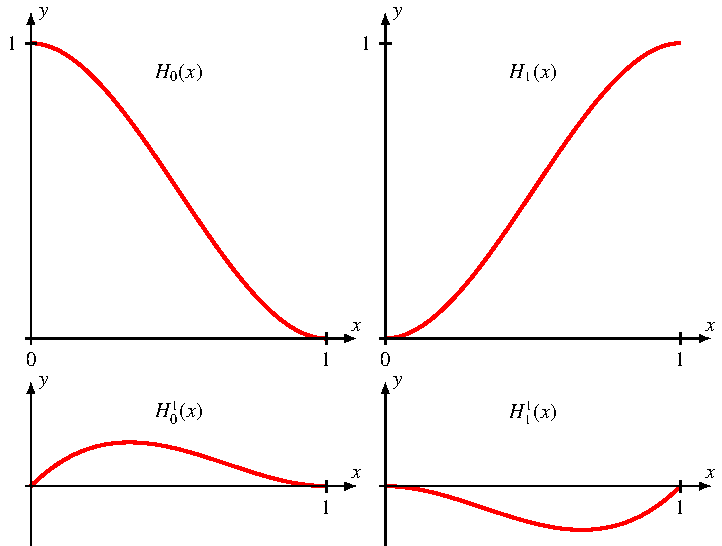
\includegraphics{chapters/30-interpolation/figures/h.pdf}
\caption{Hermite-Basispolynome für das Interval $[0,1]$
nach \eqref{buch:equation:hermite:h}
\label{buch:figure:hermite:h}}
\end{figure}
Eine besonders einfache Form nehmen die Polynome $h_j^0$ und $h_j^1$ an,
wenn man sie auf das Interval $[0,1]$ spezialisiert.
Wir bezeichnen diese Polynome mit grossen Buchstaben, sie sind
\begin{equation}
\begin{aligned}
H_0^1(x) &= x(1-x)^2=x^3-2x^2+x
&&&
H_1^1(x) &= (1-x)x^2=-x^3+x^2
\\
H_0(x)   &= (1+2x)(1-x)^2 -2x^3+5x^2-4x+1
&&&
H_1(x)   &= (3-2x)x^2 = -2x^3+3x^2
\end{aligned}
\label{buch:equation:hermite:h}
\end{equation}
Graphen dieser Polynome sind in Abbildung~\ref{buch:figure:hermite:h}
dargestellt.

Diese Polynome können auch verwendet werden, die Polynome für ein
beliebiges Intervall wieder zu gewinnen.
Dazu setzen wir $x=(x-x_0)/m$ in die Polynome ein.
Die Polynome $h_0(x)=H_0((x-x_0)/m)$ und $h_1(x)=H_1((x-x_0)/m)$
haben die Werte
\[
\begin{aligned}
h_0(x)
&=
H_0((x-x_0)/m)\bigg|_{x=x_0}
=
H_0(0)=1
&&\text{und}&
h_0(x)
&=
H_0((x-x_0)/m)\bigg|_{x=x_1}
=
H_0(1)=0
\\
h_1(x)
&=
H_1((x-x_0)/m)\bigg|_{x=x_0}
=
H_1(0)=0
&&\text{und}&
h_1(x)
&=
H_1((x-x_0)/m)\bigg|_{x=x_1}
=
H_1(1)=1
\end{aligned}
\]
und Ableitungen
\begin{align*}
h''_i(x_0)
&=
\frac{d}{dx} H_i((x-x_0)/m)\bigg|_{x=x_0}
=
H'_i((x-x_0)/m) \frac{1}{m}\bigg|_{x=x_0}
=
\frac{H_i'(0)}{m} = 0
\end{align*}
an den Intervalenden.

Tun wir dasselbe für die Polynome $H_0^1$ und $H_1^1$, erhalten wir
\begin{align*}
h_j^{1\prime}(x_i)
&=
\frac{d}{dx} H_j^1((x-x_0)/m) \bigg|_{x=x_i}
=
H_j^{1\prime}((x-x_0)/m)\bigg|_{x=x_i} \frac{1}{m}
=
\frac1m
H_j^{1\prime}(i)
=
\frac1m\delta_{ij},
\end{align*}
dies ist bis auf den Faktor $1/m$ korrekt.
Daraus lesen wir ab, dass wir die Polynome
\[
h_j^1(x)
=
mH_j^1((x-x_0)/m)
\]
für die Ableitungen verwenden müssen.

\subsubsection{Zweite Ableitungen}
Für die spätere Anwendung bei der Spline-Interpolation untersuchen
wir auch noch die zweiten Ableitung des Hermite-Interpolationspolynoms
im Fall zweier Stützstellen am Rande des Intervals.
Wir tun dies für die Polynome~\eqref{buch:equation:hermite:h}
und kümmern uns später darum, was auf anderen Intervallen passiert.
\[
\begin{aligned}
H_0''(0)                &= -6 &&&  H_0''(1)                &=  6
\\
H_1''(0)                &=  6 &&&  H_1''(1)                &= -6
\\
H_0^{1\prime\prime}(0)  &= -4 &&&  H_0^{1\prime\prime}(1)  &=  2
\\
H_1^{1\prime\prime}(0)  &= -2 &&&  H_1^{1\prime\prime}(1)  &=  4
\end{aligned}
\]
Unter Verwendung der Substition $x\to (x-x_0)/m$ können wir jetzt auch
die Werte für die zweiten Ableitungen an den Intervallenden für bestimmen.
Dazu berechnen wir erst die zweite Ableitung einer Funktion $f((x-x_0)/m)$:
\[
\frac{d^2}{dx^2} f((x-x_0)/m)
=
\frac{d}{dx} f'((x-x_0)/m) \frac1m
=
f''((x-x_0)/m) \frac1{m^2}.
\]
Angewendet auf die oben gefundenen Polynome bedeutet dies, 
\[
\begin{aligned}
h_0''(x_0) &=          - 6/m^2
&&\text{und}&
h_0''(x_1) &= \phantom{-}6/m^2 \\
h_1''(x_0) &= \phantom{-}6/m^2
&&\text{und}&
h_1''(x_1) &=          - 6/m^2 \\
h_0^{1\prime\prime}(x_0) &=           -4/m
&&\text{und}&
h_0^{1\prime\prime}(x_1) &= \phantom{-}2/m \\
h_1^{1\prime\prime}(x_0) &=          - 2/m
&&\text{und}&
h_1^{1\prime\prime}(x_1) &= \phantom{-}4/m 
\end{aligned}
\]






